\documentclass [a4paper,12pt]{article}
\usepackage{color}
\usepackage{amssymb}
\usepackage{amsmath}
\usepackage{graphicx}
\usepackage{fixltx2e}
\usepackage[
  separate-uncertainty = true,
  multi-part-units = repeat
]{siunitx}
\begin{document}
\renewcommand{\thesubsection}{\thesection.\alph{subsection}}
\begin{titlepage}
	\centering
	{\huge\bfseries Transformaciones ortogonales de  ${\rm I\!R}^2$ y ${\rm I\!R}^3$\par}
	\vspace{2cm}
	{\scshape\Large Álgebra II\par}
	\vspace{1cm}
	{\scshape\Large Universidad de Salamanca\par}
	\vspace{1cm}
	
\includegraphics[width=0.4\textwidth]
{usal}\par\vspace{1cm}
	\vspace{1.5cm}
	{\Large\itshape Manuel de la Cruz González\par}
	{\Large\itshape Cristina García Prado\par}
	{\Large\itshape Borja González Herrero\par}
	{\Large\itshape Bruno Martín González\par}
	{\Large\itshape Héctor Melchor Alaiz\par}
	{\Large\itshape Luisa del R. Montejo Fuentes\par}
	{\Large\itshape Óscar Pestañas Pérez\par}
	\vfill

% Bottom of the page
	{\large 10 de abril, 2019\par}
\end{titlepage}

%Hasta aquí la portada%
\pagenumbering{arabic}
\tableofcontents
\newpage
%Comienzo%
\section{Descripción de las ecuaciones y matrices de giros y simetrías en $\mathbb{R}^2$ y $\mathbb{R}^3$}

\subsection{Simetrías y giros en  $\mathbb{R}^2$}


La referencia ortonormal escogida en este caso es $\{0,x,y\}$ cuya base ortonormal es con base ortonormal $\{e_1,e_2\} $.

%Simetrica axial
\subsubsection{Simetría axial}
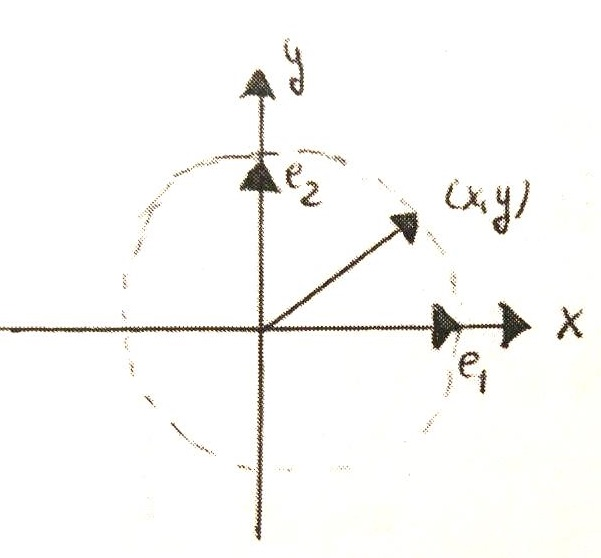
\includegraphics[width=0.4\textwidth]
{imag1}\par\vspace{1cm}
Llamaremos a este giro $S_x$ o $S_y$, según sea el eje sobre el que giro. Para el caso de $S_x$ (análogo a $S_y$) :
\begin{equation}
\begin{split}
\mathbb{R}^2\rightarrow\mathbb{R}^2 \\
(x,y)\rightarrow(x,-y)
\end{split}
\end{equation}
La matriz que describe este giro es: 
$$
S_x=\begin{pmatrix}
1&0\\
0&-1
\end{pmatrix}
$$

Si el giro es sobre el eje x, todo es análogo pero la matriz del giro en este caso es:
$$
S_y=\begin{pmatrix}
-1&0\\
0&1
\end{pmatrix}
$$
%Simetria respecto al origen
\subsubsection{Simetría respecto del origen}
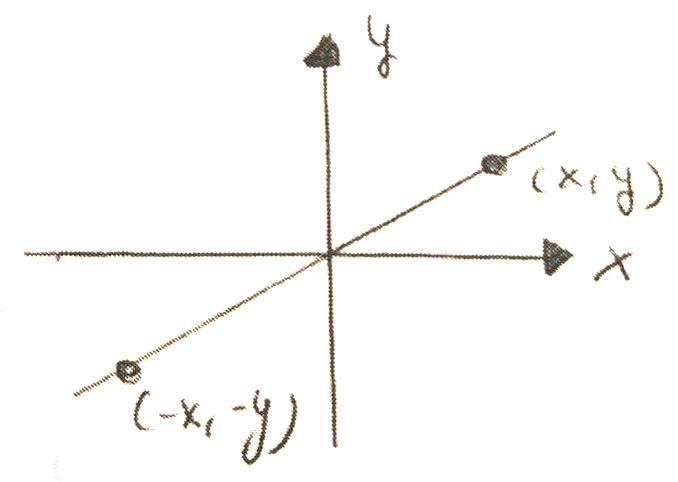
\includegraphics[width=0.4\textwidth]
{imag2}\par\vspace{1cm}
Para este caso tenemos que
\begin{equation}
\begin{split}
\mathbb{R}^2\rightarrow\mathbb{R}^2 \\
(x,y)\rightarrow(-x,-y)
\end{split}
\end{equation}
$$S_0=S_x  \circ S_y$$
Y la matriz del giro resulta en:
$$
S_0=\begin{pmatrix}
-1&0\\
0&-1
\end{pmatrix}
$$
%Giro de centro y angulo alfa
\subsubsection{Giro de centro y ángulo $\alpha$}
Sea $\{e_1,e_2\}$ una base ortonormal de $ \mathbb{R}^2$. Para un giro de ángulo 
$\alpha$ su matriz de giro asociada es:
$$
T_\alpha=\begin{pmatrix}
cos\alpha&-sen\alpha\\
sen\alpha&cos\alpha
\end{pmatrix}
$$
Las ecuaciones del giro son:
\begin{eqnarray}
T_\alpha (e_1)& = & cos\alpha  e_1 + sen\alpha  e_2 \\
T_\alpha (e_2)& = & -sen\alpha  e_1 + cos\alpha  e_2
\end{eqnarray}
Podemos comprobar que si hago el giro y a continuación hago otro giro con alfa negativa, obtengo la identidad.
$$
T_\alpha .T_{\alpha}=\begin{pmatrix}
cos^2\alpha-sen^2\alpha&-sen\alpha cos\alpha - sen\alpha cos\alpha \\
sen\alpha cos\alpha+sen\alpha cos\alpha&cos^2\alpha-sen^2\alpha
\end{pmatrix}
$$
$$
T_\alpha .T_{-\alpha}=I
$$
% PARA R3
\subsection{Simetrías y giros en  $\mathbb{R}^3$}
%giro de angulo alfa y eje de giro
\subsubsection{Giro de ángulo $\alpha$}
Ahora la matriz del giro dependerá de qué subespacio deje invariante (el eje x, el y o el z).\par
Para el eje z, el plano de giro será el xy.
$$
T_{\alpha, z}=\begin{pmatrix}
cos \alpha&- sen \alpha &0\\
sen \alpha&cos \alpha&0\\
0&0&1
\end{pmatrix}
$$
Para el eje y, el plano de giro será el zx.
$$
T_{\alpha, y}=\begin{pmatrix}
cos \alpha&0 &- sen \alpha\\
0&1&0\\
sen \alpha&0&cos \alpha
\end{pmatrix}
$$
Para el eje x, el plano de giro será el yz.
$$
T_{\alpha, x}=\begin{pmatrix}
1&0 &0\\
0&cos \alpha&- sen \alpha\\
0&sen \alpha&cos \alpha
\end{pmatrix}
$$
Para las ecuaciones, tomamos como ejemplo la del eje z:
\begin{eqnarray}
T_{\alpha, z} (e_1)& = & cos\alpha  e_1 + sen\alpha  e_2 \\
T_{\alpha, z} (e_2)& = & -sen\alpha  e_1 + cos\alpha  e_2\\
T_{\alpha, z} (e_3)&= e_3
\end{eqnarray}
Para las del eje y:
\begin{eqnarray}
T_{\alpha, y} (e_1)& = & cos\alpha  e_1 + sen\alpha  e_3 \\
T_{\alpha, y} (e_2)& =  e_2\\
T_{\alpha, y} (e_3)&= & -sen\alpha  e_1 + cos\alpha  e_3
\end{eqnarray}
Para las del eje x:
\begin{eqnarray}
T_{\alpha, x} (e_1)& = & e_1\\
T_{\alpha, x} (e_2)& = & cos\alpha  e_2 - sen\alpha  e_3 \\
T_{\alpha, x} (e_3)&= & -sen\alpha  e_2 + cos\alpha  e_3
\end{eqnarray}
Las ecuaciones son casi las mismas que para $\mathbb{R}^2$ pero con $e_3$ el subespacio que queda invariante.\par
%Simetria axial
\subsubsection{Simetría axial}
Como antes, la matriz cambiará con respecto al eje que giro.
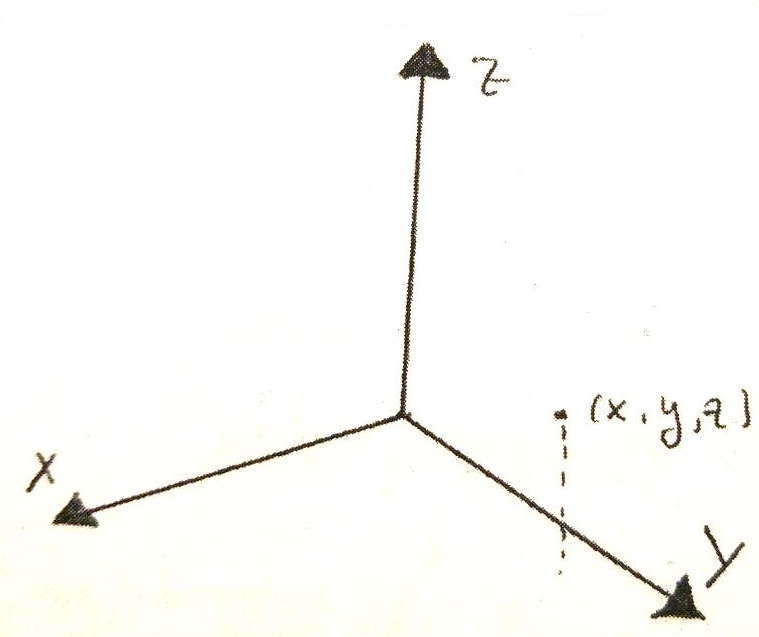
\includegraphics[width=0.4\textwidth]
{imag3}\par\vspace{1cm}
\begin{equation}
\begin{split}
\mathbb{R}^3\rightarrow\mathbb{R}^3 \\
(x,y,z)\rightarrow(x,-y,-z)/(-x,y,-z)/(-x,-y,z)
\end{split}
\end{equation}
Con respecto al eje x:
$$
S_x=\begin{pmatrix}
1&0 &0\\
0&-1&0\\
0&0&-1
\end{pmatrix}
$$
y las ecuaciones serán: 
\begin{eqnarray}
S_x(e_1)& = & e_1 \\
S_x (e_2)& = & -e_2\\
S_x (e_3)&= - e_3
\end{eqnarray}
Con respecto al eje y:
$$
S_y=\begin{pmatrix}
-1&0 &0\\
0&1&0\\
0&0&-1
\end{pmatrix}
$$
y las ecuaciones serán: 
\begin{eqnarray}
S_y(e_1)& = & -e_1 \\
S_y (e_2)& = & +e_2\\
S_y (e_3)&= - e_3
\end{eqnarray}
Con respecto al eje z:
$$
S_z=\begin{pmatrix}
-1&0 &0\\
0&-1&0\\
0&0&1
\end{pmatrix}
$$
y las ecuaciones serán: 
\begin{eqnarray}
S_z(e_1)& = & -e_1 \\
S_z (e_2)& = & -e_2\\
S_z (e_3)&= e_3
\end{eqnarray}
Esta simetría también recibe el nombre de especular.
%simetria con respecto el origen
\subsubsection{Simetría con respecto el origen}
En este caso, tanto x como y y z cambiarán de signo.
$$
S_0=\begin{pmatrix}
-1&0 &0\\
0&-1&0\\
0&0&-1
\end{pmatrix}
$$
y sus ecuaciones asociadas
\begin{eqnarray}
S_z(e_1)& = & -e_1 \\
S_z (e_2)& = & -e_2\\
S_z (e_3)&= -e_3
\end{eqnarray}
%APARTADO B
\section{Demostración de ortogonalidad}
Para demostrar que son ortogonales debemos comprobar que el producto de la matriz de giro por su traspuesta nos devuelve la identidad.\par
También, el determinante de una matriz ortogonal debe de ser $\pm1$.\par
Además, los únicos valores propios posibles para una aplicación ortogonal son $\pm1$.

\subsection{En  $\mathbb{R}^2$}
%siemtria axial
\subsubsection{Simetría axial}
La matriz que describe este giro es: 
$$
S_x=\begin{pmatrix}
1&0\\
0&-1
\end{pmatrix}
$$
Podemos ver que es un isomorfismo de valor propio 1 y -1 ya que descompone diagonalmente con esos valores. Podemos también observar que al aplicarla dos veces, obtenemos el estado inicial ya que:
$$ S_x^2=I$$
Con esto hemos demostrado que es ortogonal ya que la matriz de giro y su traspuesta es la misma.
La demostración es igual para el caso del eje y. \par
Es claro que el determinante de $S_x$ y $S_y$ es $-1$ y que sus valores propios son $\pm1$.
%siemtria respecto al origen
\subsubsection{Simetría respecto del origen}
La matriz del giro es:
$$
S_0=\begin{pmatrix}
-1&0\\
0&-1
\end{pmatrix}
$$
Como $S_0=S^t_0$:
$$
S_0.S^t_0=S^2_0=I
$$
y $det S_0=+1$\par
Los valores propios de esta matriz son $\pm1$

%giro de centro y angulo alfa
\subsubsection{Giro de centro y ángulo $\alpha$}
Para un giro de ángulo 
$\alpha$ su matriz de giro asociada es:
$$
T_\alpha=\begin{pmatrix}
cos\alpha&-sen\alpha\\
sen\alpha&cos\alpha
\end{pmatrix}
$$
Hacemos el producto con su traspuesta y obtenemos:
$$
T_\alpha .T^t_{\alpha}=\begin{pmatrix}
cos^2\alpha+sen^2\alpha&-sen\alpha cos\alpha + sen\alpha cos\alpha \\
sen\alpha cos\alpha-sen\alpha cos\alpha&cos^2\alpha+sen^2\alpha
\end{pmatrix}= I
$$
$$
T_\alpha .T^t_{\alpha}=I
$$
Si hacemos su determinante:
$det T_\alpha = cos^2\alpha+sen^2\alpha = 1$\par
Vamos a proceder ahora a calcular el determinante.
$$
\begin{vmatrix}
x-cos\alpha&sen\alpha\\
-sen\alpha&x-cos\alpha
\end{vmatrix}=x^2-2 cos\alpha x +1
$$
$$
x=\frac{2 cos\alpha \pm \sqrt{4 cos^2 \alpha -4}}{2}=cos \alpha \pm \sqrt{cos^2\alpha -1}
$$
Por tanto alfa sólo puede 180º o 0º para valores propios reales. Entonces:
$$x=cos 0º=1$$ o
$$x=cos 180º=-1$$
%EN R3
\subsection{En  $\mathbb{R}^3$}
%Giro angulo 
\subsubsection{Giro de ángulo $\alpha$}
La matriz para el eje z es
$$
T_{\alpha, z}=\begin{pmatrix}
cos \alpha&- sen \alpha &0\\
sen \alpha&cos \alpha&0\\
0&0&1
\end{pmatrix}
$$
y su traspuesta :
$$
T^t_{\alpha, z}=\begin{pmatrix}
cos \alpha&+sen \alpha &0\\
-sen \alpha&cos \alpha&0\\
0&0&1
\end{pmatrix}
$$
El producto de ambas 
$$
T_{\alpha, z} .T^t_{\alpha, z}=\begin{pmatrix}
cos^2\alpha+sen^2\alpha&-sen\alpha cos\alpha + sen\alpha cos\alpha &0\\
sen\alpha cos\alpha-sen\alpha cos\alpha&cos^2\alpha+sen^2\alpha&0\\
0&0&1
\end{pmatrix}= I
$$
El determinante lo puedo calcular desarrollando por el menores (tomo el 1) y obtengo por tanto el mismo determinante que para la matriz de giro de $\mathbb{R}^2$.\par
$ det T_{\alpha, z} = 1$ \par
Procedemos al cálculo de los valores propios
$$
\begin{vmatrix}
x-cos\alpha&sen\alpha&0\\
-sen\alpha&x-cos\alpha&0\\
0&0&x-1
\end{vmatrix}=(x-1)\begin{vmatrix}
x-cos\alpha&sen\alpha\\
-sen\alpha&x-cos\alpha
\end{vmatrix}
$$
Donde el segundo determinante es el que hemos calculado antes para $\mathbb{R}^2$. Por tanto, queda demostrado que sólo puede tener como valores propios $\pm1$.
%axial y respecto al origen
\subsubsection{Simetría axial y respecto al origen}
Como las matrices son diagonales, sus traspuestas coinciden con la matrices.
Es secillo ver que las matrices: 
$
S_x=\begin{pmatrix}
1&0 &0\\
0&-1&0\\
0&0&-1
\end{pmatrix}
$
$
S_y=\begin{pmatrix}
-1&0 &0\\
0&1&0\\
0&0&-1
\end{pmatrix}
$
$
S_z=\begin{pmatrix}
-1&0 &0\\
0&-1&0\\
0&0&1
\end{pmatrix}
$
Al elevarlas al cuadrado, obtengo la identidad, ya que los signos desaparecen.\par
También podemos ver a simple vista que el determinante de todas ellas es 1.\par
Para el caso de la simetría respecto el origen, lo anteriormente dicho es válido; pero el determinante de esta es -1.
$$
S_0=\begin{pmatrix}
-1&0 &0\\
0&-1&0\\
0&0&-1
\end{pmatrix}
$$
Como todas son matrices diagonales, sabemos por el Primer Teorema de descomposición que los únicos valores propios posibles son aquellos que se encuentran en la diagonal y por tanto, $\pm1$.
%PARTE C
\section{Demostración propuesta}
Demostrar que si T es una transformación ortogonal, existe una base ortonormal respecto de la que T es expresable como composición de giros y simetrías.	\par

\textbf{Demostración}

Partimos de las siguientes condiciones:
\begin{enumerate}
\item Como t es una transformación ortogonal, los calores propios que puede tener son $\pm1$.
\item Si existe una base ortonormal, la matriz asociada a T es Id y por tanto $$A^t . A=Id\rightarrow A^t=A^{-1}$$
\item Se sabe, además, que el determinante de A tiene que ser $\pm1$.
\end{enumerate}
Como resultado de todo lo enumerado la matriz T asociada a la transformación ortogonal respecto a una base B ortonormal es semejante a:
$$
T_B=\begin{pmatrix}
\pm1& &\\
&\pm1&\\
&&\ddots\\
&&&\pm1
\end{pmatrix}
$$
\begin{itemize}
\item[+] En caso de ser todos -1 tenemos simetría en el origen.
\item[+] Con un +1 tenemos simetría respecto los ejes.
\item[+] Si sólo tengo 1, tendríamos la matriz identidad.
\end{itemize}
Particularizando para $\mathbb{R}^3$. Las posibilidades de giro son, en base a lo anterior, las matrices de giro que hemos expresado en el apartado a).
$$
T_{\alpha, z}=\begin{pmatrix}
cos \alpha&\pm sen \alpha &0\\
\pm sen \alpha&cos \alpha&0\\
0&0&\pm1
\end{pmatrix}
$$
Para el eje y, el plano de giro será el zx.
$$
T_{\alpha, y}=\begin{pmatrix}
cos \alpha&0 & \pm sen \alpha\\
0&\pm1&0\\
\pm sen \alpha&0&cos \alpha
\end{pmatrix}
$$
Para el eje x, el plano de giro será el yz.
$$
T_{\alpha, x}=\begin{pmatrix}
\pm1&0 &0\\
0&cos \alpha&\pm sen \alpha\\
0&\pm sen \alpha&cos \alpha
\end{pmatrix}
$$
%END
\begin{flushleft}
\end{flushleft}
\end{document}